\documentclass[air,article,submit,moreauthors]{Definitions/mdpi}

\firstpage{1}
\makeatletter
\setcounter{page}{\@firstpage}
\makeatother
\pubvolume{1}
\issuenum{1}
\articlenumber{0}
\pubyear{2026}
\copyrightyear{2026}
\datereceived{ }
\daterevised{ }
\dateaccepted{ }
\datepublished{ }

\Title{Short-Window Response of WRF Cold-Pool Retention to Driving Data and Nest Feedback during a Uinta Basin Winter-Ozone Episode}

\newcommand{\orcidauthorA}{0000-0003-0305-4090}
\newcommand{\orcidauthorB}{0009-0009-9083-6568}
\newcommand{\rewritegate}[1]{\textbf{[Rewrite gate: #1]}}
\Author{John R. Lawson $^{1,2,}$*\orcidA{}, Michael J. Davies $^{1}$\orcidB{}, Loknath Dhar $^{1,3}$ and Seth N. Lyman $^{1,3}$}
\AuthorNames{John R. Lawson, Michael J. Davies, Loknath Dhar and Seth N. Lyman}

\address{%
$^{1}$ \quad Bingham Research Center, Utah State University, Vernal, UT 84078, USA;\\
$^{2}$ \quad Department of Mathematics and Statistics, Utah State University, Logan, UT 84322, USA;\\
$^{3}$ \quad Department of Chemistry and Biochemistry, Utah State University, Logan, UT 84322, USA}
\corres{Correspondence: john.lawson@usu.edu}

\abstract{A winter-ozone chemistry model receives a finite mixing volume and wind field from its meteorological driver, but conventional surface scores do not establish whether that driver preserves a shallow, weakly ventilated lower layer.
We tested four deterministic Weather Research and Forecasting (WRF) simulations of the 2 February 2013 Uinta Basin episode in a two-by-two design that crossed GFS and NAM driving-data products with one-way and two-way nest feedback.
The common evaluation used eleven fixed station columns on the 1 km domain and five post-spin-up hours from 14:00 to 18:00 UTC.
Relative to NAM, GFS increased the paired 2 m-temperature-bias contrast by 1.79 and 1.76~$^{\circ}$C under two-way and one-way feedback, respectively.
GFS-minus-NAM 50--500 m above-ground-level potential-temperature stability was -3.63 and -3.65 K, while fixed-layer transport wind was +0.79 and +0.99 m s$^{-1}$.
Both lower-layer contrasts retained the same sign in all five hours under both feedback modes.
The within-product feedback effects were much smaller for the same diagnostics.
These simulations therefore supplied distinct short-window lower-layer states despite the feedback choice, but the experiment does not isolate initial from boundary forcing, validate inversion depth, establish multi-day persistence, calculate basin export, or predict ozone.}

\keyword{winter ozone; WRF; cold-air pool; Uinta Basin; driving data; nest feedback; model evaluation}

\begin{document}

\section{Introduction}

Winter ozone in the Uinta Basin develops when photochemistry proceeds within snow-covered, stably stratified air that restricts vertical dilution and horizontal exchange.
Snow, radiation, deposition, emissions, chemistry, and transport all participate in the observed response \citep{Ahmadov2015-zm,Neemann2015-ws,Davies2025-wy}.
For a coupled model, the meteorological question is therefore not only whether 2 m temperature has a small mean error.
It is whether the atmosphere delivered to the chemistry grid contains a credible shallow mixing environment and weak transport during the accumulation period.

Published concentration agreement does not provide a clean ranking of the relevant uncertainties.
Ahmadov et al. obtained a much stronger ozone simulation with a top-down oil-and-gas inventory, while also conditioning inventory interpretation on adequate meteorology \citep{Ahmadov2015-zm}.
Matichuk et al. found substantial emissions and deposition sensitivities, but improved WRF temperature profiles did not consistently improve ozone profiles \citep{Matichuk2017-bq}.
These outcomes are consistent with compensating error among confinement, emissions, photolysis, deposition, and chemical mechanism.
They make meteorological evaluation necessary for chemical attribution without making meteorology the uniquely dominant error source.

The meteorological literature also warns against reducing an experiment to a configuration label.
Neemann et al. showed strong case-specific responses to snow and cloud treatment, but their ice-retention modification was a bounding treatment and the grid evaluated most closely was finer than the grid supplied to the chemistry model \citep{Neemann2015-ws}.
Tran et al. showed that the response to four-dimensional data assimilation depended on the nudged variables, input data, and diagnosed boundary-layer depth \citep{Tran2018-cx}.
Thus, labels such as ``NAM driven,'' ``nudged,'' or ``high resolution'' do not by themselves identify a controlled cause, and aggregate scores can obscure a failure to retain the layer of interest.

The present study asks two deliberately bounded questions.
First, does the short-window lower-layer state differ between GFS- and NAM-driven WRF simulations under both nest-feedback modes?
Second, how large is the within-product nest-feedback response relative to that driving-product contrast?
We answer these questions with paired surface errors and common-height stability and wind diagnostics on one domain, station field, and five-hour window.
The design evaluates the meteorological input state that a later chemistry calculation would receive; it does not contain a chemistry calculation.

\section{Materials and Methods}

\subsection{Factorial Design and Estimands}

The experiment crossed the archived GFS analysis product \texttt{gfsanl\_4} and NAM analysis product \texttt{namanl\_218} with one-way and two-way nest feedback (Table~\ref{tab:test-matrix}).
Stable study codes connect each member to the run and comparison inventories.
The two product contrasts were evaluated separately so that the driving-product response had to recur under both feedback settings to support the primary result.
The two within-product feedback contrasts and their paired interaction bounded the secondary response.

\begin{table}[H]
\caption{Driving-product by nest-feedback experiment matrix.
The study codes resolve to exact run paths and fingerprints in the run inventory.}
\label{tab:test-matrix}
\centering
\begin{tabular}{llll}
\toprule
Study code & Driving-data product & Nest feedback & Manuscript label \\
\midrule
X6  & GFS & two-way & GFS two-way \\
X10 & GFS & one-way & GFS one-way \\
X5  & NAM & two-way & NAM two-way \\
X3  & NAM & one-way & NAM one-way \\
\bottomrule
\end{tabular}
\end{table}

The GFS-versus-NAM factor is a product-level treatment.
It bundles the products' native grids, analysis systems, vertical input, assimilated observations, 12:00 UTC initial state, and subsequent lateral-boundary evolution.
The experiment cannot assign the resulting response to one of those components.
Within each product family, the normalized as-run namelists differed only in the feedback flag.

\subsection{Case, Observations, and Common Sample}

The target is the snow-covered Uinta Basin cold-air pool on 2 February 2013 within the episode examined by prior meteorological and chemical studies \citep{Neemann2015-ws,Ahmadov2015-zm}.
All factorial comparisons use 14:00--18:00 UTC, corresponding to 07:00--11:00 mountain standard time.
The first two forecast hours were excluded as spin-up, leaving five hourly samples.

Surface observations were extracted from the Synoptic archive for eleven stations reporting 2 m temperature, ten reporting 10 m wind speed, and nine reporting surface pressure in every retained hour.
Subhourly reports were averaged within each UTC clock hour.
The stations span basin-floor, sidewall, and bench locations but are neither spatially uniform nor area weighted.
The 1 km second domain, d02, was selected because the 333 m third domain excludes most higher bench stations.

Four elevation-spanning stations provide surface context from 31 January 00:00 UTC through 4 February 00:00 UTC.
Their separation is a spatial surface-temperature pattern, not a colocated free-air profile.
No sounding, profiler, or remote-sensing profile is used to validate the modeled 50--500 m layer.

\rewritegate{Document the Synoptic citation and access date, API quality-control parameters, station ownership, sensor heights and metadata, completeness screening, observation uncertainty, public-access route, and archive license.}

\subsection{WRF Configuration}

The four free forecasts used WRF version 4.8.0 from 12:00 to 18:00 UTC on 2 February 2013.
Three nested domains had horizontal grid spacing of 3, 1, and 0.333 km, 75 eta levels, and a 50 hPa model top.
The common physics suite used Thompson microphysics, RRTMG longwave and shortwave radiation, the revised MM5 surface layer, the Noah land-surface model, and the YSU planetary-boundary-layer scheme.
Grid and observation FDDA were disabled.
The runs shared domain geometry, default 30-arc-second-class terrain, physics, initialization time, output cadence, and valid window.
The GFS one-way member reused the verified GFS two-way metgrid files before rerunning \texttt{real.exe} and \texttt{wrf.exe}.

\rewritegate{Add the WRF and exact GFS/NAM product citations, map projection, domain dimensions and centers, time step, boundary interval, static-geography versions, and snow-field initialization from the archived as-run records.}

\subsection{Surface and Common-AGL Diagnostics}

Modeled 2 m temperature, earth-relative 10 m wind, and surface pressure were sampled at the nearest d02 cell to each station.
Across the eleven fixed columns, model terrain minus station elevation had a median of -2.0 m and ranged from -32.4 to +14.3 m.
That agreement limits one obvious mismatch but does not remove exposure, slope, land-cover, or network-coverage error.

Mass-level height above ground was calculated from perturbation and base-state geopotential and the local WRF terrain height.
Grid-relative winds were destaggered and rotated to earth-relative components.
Potential temperature and both wind components were interpolated linearly at 25 m increments from 50 to 500 m above ground level (AGL) at each station column.
Fixed-layer stability was defined as $S_{50:500}=\theta(500\,\mathrm{m})-\theta(50\,\mathrm{m})$.
The transport-wind proxy was $U_{50:500}=\{\bar{u}^{2}+\bar{v}^{2}\}^{1/2}$, where the bars denote height means from 50 to 500 m AGL.
This wind metric is not flow through the basin boundary, pollutant residence time, cold-pool volume, or a chemistry-model ventilation coefficient.
Native WRF PBL height was retained only as a scheme-dependent companion diagnostic.

\subsection{Pairing, Aggregation, and Short-Sample Scope}

Run differences were paired by station and valid hour before spatial aggregation.
The forcing-by-feedback interaction was defined as
$[\mathrm{GFS}_{1\mathrm{w}}-\mathrm{GFS}_{2\mathrm{w}}]-[\mathrm{NAM}_{1\mathrm{w}}-\mathrm{NAM}_{2\mathrm{w}}]$.
Each station field was reduced to one unweighted spatial median per hour, and the five hourly medians were averaged for the reported effect.
The stations were not treated as independent replicates.

Hourly ranges and sign counts describe temporal consistency directly.
A two-hour circular moving-block calculation and leave-one-hour-out ranges were retained in the reproducibility record as descriptive sensitivity checks.
They are not confidence intervals, hypothesis tests, or estimates of observation, forcing, or structural uncertainty.
No population inference is attempted from four deterministic integrations of one case.

\section{Results}

\subsection{Observed Surface Context}

The basin-floor station at Pariette Draw repeatedly cooled below the higher sites from 31 January through 3 February, while the magnitude and ordering of the station temperatures changed through the diurnal cycle (Figure~\ref{fig:test-observed}).
The recurring floor-to-bench separation is consistent with cold-pool conditions around the modeled period.
It does not determine the cold-pool top, depth, volume, or basin-wide energy deficit.

\begin{figure}[H]
\centering
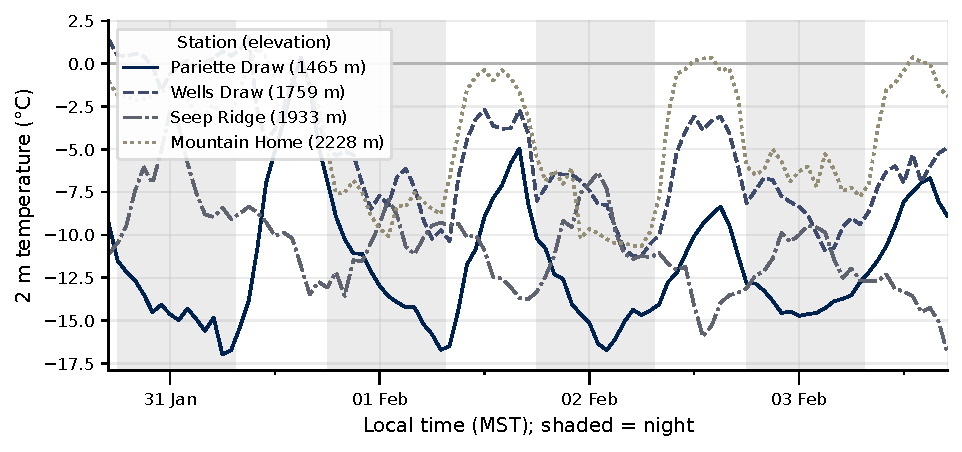
\includegraphics[width=\textwidth]{figures/obs_temp_timeseries_feb0102.pdf}
\caption{Observed 2 m-temperature evolution at four elevation-spanning Uinta Basin stations from 31 January through 3 February 2013.
Shading indicates approximate local night.
The sites establish a recurring spatial surface-temperature pattern but do not constitute a colocated vertical profile.}
\label{fig:test-observed}
\end{figure}

\subsection{Driving-Product Response Reproduced across Feedback Modes}

The common-AGL diagnostics separated the driving products under both feedback settings (Figure~\ref{fig:test-retention}).
GFS minus NAM reduced 50--500 m potential-temperature stability by 3.63 K under two-way feedback and 3.65 K under one-way feedback (Table~\ref{tab:test-effects}).
The five hourly spatial-median differences ranged from -5.58 to -1.13 K and from -5.36 to -0.90 K, respectively.
All ten product-by-hour stability contrasts therefore retained the same sign.

GFS minus NAM increased fixed-layer transport wind by 0.79 m s$^{-1}$ under two-way feedback and 0.99 m s$^{-1}$ under one-way feedback.
The hourly differences ranged from +0.37 to +1.18 m s$^{-1}$ and from +0.61 to +1.50 m s$^{-1}$, with the same sign in every hour.
Native PBL-height differences changed sign within both feedback modes and did not reproduce the stability and wind separation.

\begin{figure}[H]
\centering
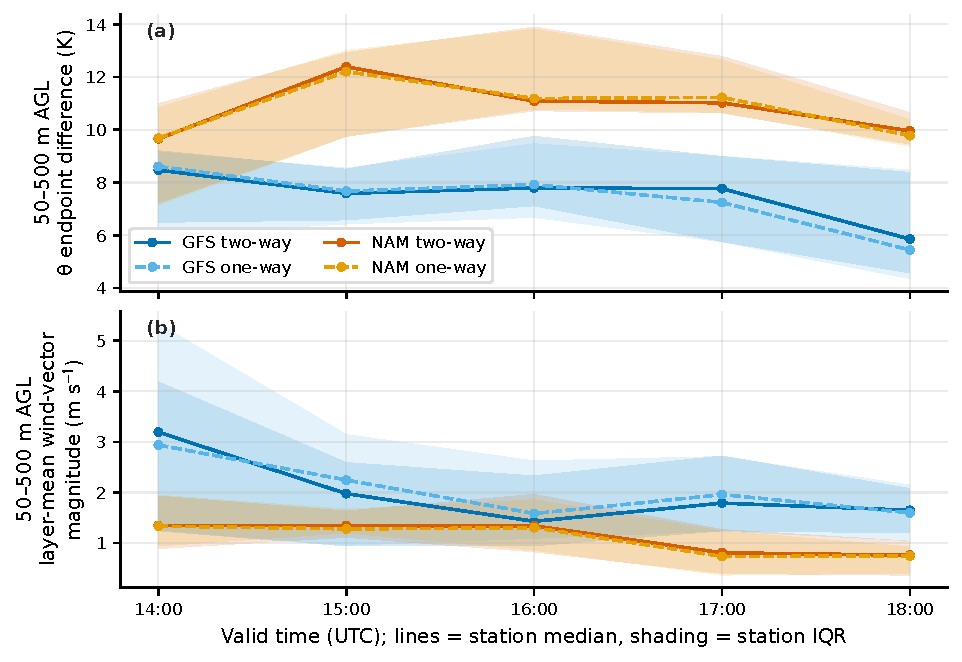
\includegraphics[width=\textwidth]{figures/wrf_retention_ventilation_d02_14to18.pdf}
\caption{Station-column medians and interquartile ranges for 50--500 m AGL potential-temperature stability, fixed-layer transport wind, and native WRF PBL height over the matched window.
Solid lines denote two-way feedback and dashed lines denote one-way feedback.
The lower-layer GFS--NAM separation recurs under both feedback modes, while PBL height is retained as a scheme-dependent companion rather than an observed layer depth.}
\label{fig:test-retention}
\end{figure}

\begin{table}[H]
\caption{Paired effects averaged over five hourly spatial medians.
Positive T2 values indicate a warmer model-minus-observation bias, positive stability values indicate a more stable fixed layer, and positive transport-wind values indicate a larger fixed-layer wind.
The values are deterministic descriptive contrasts.}
\label{tab:test-effects}
\centering
\begin{tabular}{lrrr}
\toprule
Effect & $\Delta$T2 bias ($^{\circ}$C) & $\Delta S_{50:500}$ (K) & $\Delta U_{50:500}$ (m s$^{-1}$) \\
\midrule
GFS $-$ NAM, two-way & +1.79 & -3.63 & +0.79 \\
GFS $-$ NAM, one-way & +1.76 & -3.65 & +0.99 \\
GFS one-way $-$ two-way & +0.07 & -0.07 & +0.10 \\
NAM one-way $-$ two-way & -0.01 & +0.00 & +0.01 \\
Feedback interaction & +0.04 & -0.10 & +0.10 \\
\bottomrule
\end{tabular}
\end{table}

\subsection{Surface Corroboration and the Feedback Bound}

The paired surface-temperature result had the same product ordering.
GFS minus NAM increased the hourly station-median 2 m-temperature-bias contrast by 1.79~$^{\circ}$C under two-way feedback and 1.76~$^{\circ}$C under one-way feedback.
The corresponding absolute-error differences were +1.41 and +1.50~$^{\circ}$C.
The surface result corroborates the lower-layer separation but does not substitute for it.

Within each product, the feedback response was much smaller than the GFS-minus-NAM response.
GFS one-way minus two-way averaged -0.066 K in stability and +0.104 m s$^{-1}$ in transport wind.
NAM one-way minus two-way averaged +0.002 K and +0.006 m s$^{-1}$ for the same metrics.
The paired interaction was -0.103 K for stability and +0.097 m s$^{-1}$ for transport wind.
These values bound the response of the present configuration and sample; they do not establish general equivalence between feedback modes.

\section{Discussion}

\subsection{A Product-Level Difference, Not a Universal Product Ranking}

The principal result is a replicated product-level separation.
The GFS-driven members are warmer at the evaluated surface sites, less stable across the fixed 50--500 m layer, and faster in the fixed-layer transport metric than the NAM-driven members under both feedback settings.
Replication across the feedback flag makes this ordering insensitive to that one configuration choice within the present experiment.
It does not establish that NAM is generally superior or that a single property of GFS caused the response.

The product factor combines the 12:00 UTC initial atmosphere with boundary updates through 18:00 UTC.
A direct comparison of each product with an independent profile at initialization would test inherited lower-tropospheric error.
A further experiment that holds either the initial or boundary state fixed would be needed to apportion the subsequent response.
Until those tests exist, ``driving-product response'' is more accurate than ``initial-condition effect.''

\subsection{What the Difference Means for an Air-Quality Model}

The GFS members supplied a less stable and faster-moving 50--500 m layer over the fixed station columns.
That combination is consistent with a meteorological state more favorable to dilution than the matched NAM state.
The distinction is relevant because a chemistry calculation cannot recover a shallow accumulation volume that is absent from its meteorological input.
However, the present transport-wind metric does not measure pollutant export, and no chemical species were simulated.

This boundary is important in the Uinta Basin literature.
Inventory changes, snow-enhanced photolysis, deposition, chemical mechanisms, and meteorological confinement have all produced substantial, interacting responses \citep{Ahmadov2015-zm,Neemann2015-ws,Matichuk2017-bq}.
An improved meteorological state need not yield improved ozone if another component changes or compensates.
The present result therefore identifies a meteorological precondition for attribution rather than assigning an ozone effect or ranking all sources of model error.

\subsection{Why the Common-AGL Result Leads the Paper}

The rewrite gives the common-AGL panel priority over a two-site bulk potential-temperature contrast.
The latter is useful descriptive context, but its stations are horizontally separated and only its two-way product pair is shown.
It cannot validate a free-air inversion.
By contrast, the common-AGL calculation applies the same geometric layer, fixed columns, valid times, and aggregation to all four simulations and directly displays both experimental factors.

Native PBL height is not a replacement for that calculation.
Its product contrasts changed sign, and its physical meaning depends on the boundary-layer scheme.
This behavior follows the broader lesson from data-assimilation and cold-pool studies that diagnosed PBL depth, nudging reach, and chemistry-grid structure must be disclosed rather than treated as interchangeable \citep{Tran2018-cx,Neemann2015-ws}.

\subsection{Limits That Determine the Next Experiment}

The five-hour window is the strongest limit.
It can show a coherent short-window separation but cannot establish multi-day retention, event buildup, or cold-pool breakup.
The two-hour spin-up exclusion has not been varied, and resampling five dependent hourly medians cannot create an inferential sample.

The observation network creates a second limit.
Four stations establish surface context and eleven fixed columns support matched comparisons, but neither set observes the modeled vertical layer.
Small nearest-cell elevation errors do not remove exposure and representativeness error.
Independent in-basin vertical observations are required to evaluate inversion depth and common-AGL stability directly.

The next discriminating sequence is therefore to verify observation provenance and full model configuration, extend the same factorial through a longer matched window, add an independent vertical reference, and separate initial from boundary-state contributions.
Only after those steps should selected meteorological states be crossed with emissions and chemical mechanisms in a coupled attribution experiment.
Archived terrain, PBL, resolution, and nudging families remain separate controlled questions or heterogeneous context rather than additional evidence for the present result.

\section{Conclusions}

Four specific WRF simulations show a coherent five-hour response to the driving-data product on the common d02 station-column sample.
Relative to NAM, GFS is warmer at the surface, less stable from 50 to 500 m AGL, and faster in the fixed-layer transport-wind metric under both one-way and two-way nest feedback.
The within-product feedback responses are much smaller for those diagnostics.
The result establishes a short-window difference in the meteorological state available to downstream chemistry; it does not identify the responsible product component, validate inversion depth, demonstrate event-scale persistence, calculate basin ventilation, or predict ozone.

\vspace{6pt}

\authorcontributions{\rewritegate{Assign and approve CRediT roles for all authors.}}
\funding{\rewritegate{Insert verified funders and grant numbers.}}
\institutionalreview{Not applicable.}
\informedconsent{Not applicable.}
\dataavailability{The analysis scripts, derived summaries, run and comparison inventories, and promoted figures used for this experimental rewrite are retained in the private working repository.
\rewritegate{Add a public repository or DOI, licenses and access conditions for raw WRF and Synoptic data, and the exact release commit before submission.}}
\acknowledgments{\rewritegate{Identify computational facilities, data providers, and contributors who do not meet the authorship criteria.}}
\conflictsofinterest{\rewritegate{All authors must confirm the conflicts-of-interest statement.}}
\useofartificialintelligence{Generative artificial intelligence tools, including Anthropic Claude and OpenAI Codex, were used during manuscript preparation to assist with literature synthesis, provenance and analysis-code review, and drafting and editing.
The authors reviewed and edited the resulting material and take responsibility for the content.}

\begin{adjustwidth}{-\extralength}{0cm}
\reftitle{References}
\bibliography{paperpile}
\PublishersNote{}
\end{adjustwidth}

\end{document}
